\chapter{Prolegomena}
\label{chap:prolegomena}
%DGW: prolegomena is the plural form of prelogmenon, but in any case I would recommend "Introduction" over an ancience greek term ;)

\section{Reinforcement Learning: what is an MDP?}

A \textbf{Markov Decision Process} \cite{mdp} (or \textit{MDP}) is a process that formally describes a fully-observable environment, which means the current state fully characterizes the environment. 

It can be defined as:

\begin{itemize}
    \item a set of states $S$
    \item a set of actions $A$ that can be taken from the states in $S$
    \item the probability $P_a(s, s')$ of reaching each state $s'$ if action $a$ is chosen from state $s$
    \item and the immediate reward $R_a(s, s')$ associated with transitioning from state $s$ to state $s'$ by taking actions $a$
\end{itemize}

An environment can be considered to have a \textbf{sparse reward}, which means many transitions between states have the same null reward, and only a few have a different information. This raises the issue of reward plateaus, where there is no information on what makes an action better than the others, hence making it harder to evaluate a state.

An example of environments with sparse rewards are games like chess, where only winning or losing give tangible information on the value of a state, but not intermediate game states. Hence, an agent can play many steps without receiving any reward, and will need to explore many trajectories to find information.
      
\begin{figure}[H]
    \centering
    \begin{tikzpicture}
  \node[draw] (A) at (0cm,0cm) {State s + Action s};
  \node[draw] (B) at (3cm,1.5cm) {State s'};
  \node[draw] (C) at (3cm,-1.5cm) {State s''};

  
  \node[draw,fill=yellow] (Arga) at (1.5cm,2.5cm) {Proba $p_1$};
  \node[draw,fill=yellow] (Argb) at (1.5cm,-2.5cm) {Proba $p_2$};
  
  \draw node[vertex] (Jointa) at (1.5cm,0.75cm) {};
  \draw node[vertex] (Jointb) at (1.5cm, -0.75cm) {};
  
  \draw[->,draw=blue] (A) to (B);
  \draw[->,draw=blue] (A) to (C);
  
  \draw[-,draw=black] (Arga) to (Jointa);
  \draw[-,draw=black] (Argb) to (Jointb);
  
  \end{tikzpicture}
  
    \caption{Markov Decision Process ($p_1 + p_2 = 1$)}
    \label{fig:my_label}
\end{figure}

A (deterministic) \textbf{policy} $\pi$ is a mapping from states to actions. $\pi: S \longrightarrow A$.

The goal of \textbf{Reinforcement Learning} is to find the optimal policy $\pi^*$ that maximizes the expected sum of rewards across an experiment. 
% DGW: write this theoretically and include a few more citations

\section{Artificial Neural Networks acting as a policy}
% DGW: What is a Neural Network? (should be Artificial Neural Network throughout) what are weights, biases, architecture? Needs to be explained, a visualization would help

\subsection{Artificial Neural Networks}

An Artificial Neural Network (or \textit{ANN}, simply called Neural Network in this document) is a bio-inspired computing systems based on some principles present in the biological brain. ANNs can be represented as a directed graph of artificial neurons connected to each other. 

An artificial neuron is a simple computing unit which effectuates a weighted sum of multiple inputs $x_i$, adds a bias $b$, and then computes a function (called \textit{activation function} $f$) on this sum. The final value is presented as output $Y$:

\begin{equation*}
\label{eq:neuron}
 Y = f(\sum_i w_i x_i + b)
\end{equation*}
with $w_i$ the weight associated with input $i$ (cf figure \ref{fig:neuron}).

\begin{figure}[H]
 \centering
 \captionsetup{justification=centering, margin=0.5cm}
 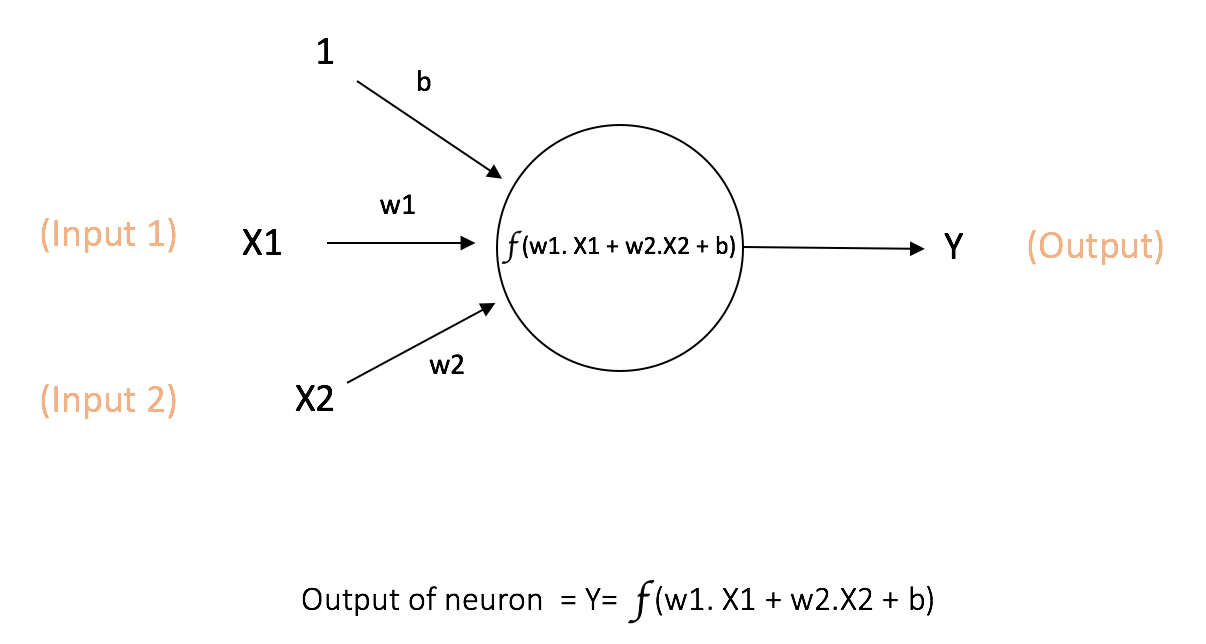
\includegraphics[width=10cm]{images/neuron.png}
 \caption{Representation of an Artificial Neuron}
\small\textsuperscript{\url{https://www.kdnuggets.com/2016/11/quick-introduction-neural-networks.html}}
 \label{fig:neuron}
\end{figure}

As illustrated in figure \ref{fig:ann}, ANNs are functions in which input neurons each take the value of an argument, and the output of the function is a vector computed from the concatenation of the values of the output neurons.

Traditionally, neurons are presented as layers in an ANN, units of a layer taking the outputs of neurons of the previous layer as input, and being used by the next layer. Each layer is then computed successively, from the input layer to the output. Recurrent units link the output of neurons to the input of earlier neurons, transmitting information from an evaluation to the next one, which can be useful for series of linked data points. 

If this structure is convenient to represent fixed networks, other architectures can exist where each neuron is considered individually and can be linked to any other neuron, without layers. These architectures however require a specific heuristic defining the order in which all neurons are computed.

\begin{figure}[H]
 \centering
 \captionsetup{justification=centering, margin=0.5cm}
 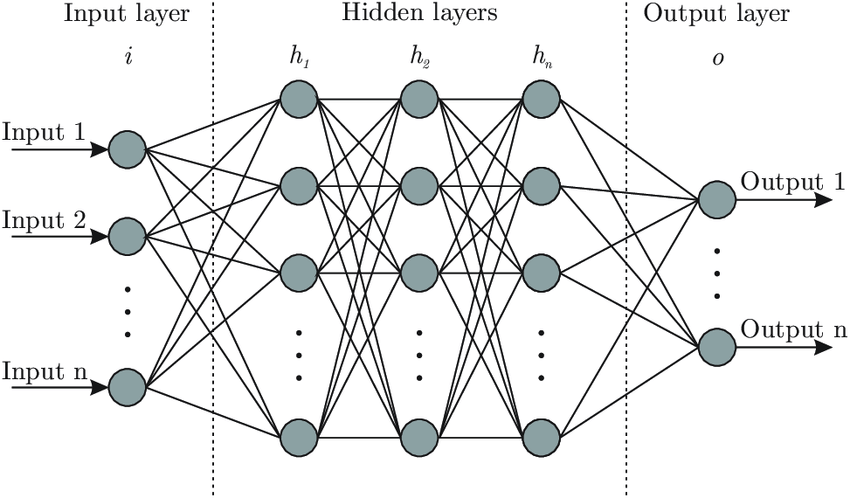
\includegraphics[width=10cm]{images/Artificial-neural-network-architecture-ANN-i-h-1-h-2-h-n-o.png}
 \caption{Representation of an Artificial Neural Network with layers in \cite{ann-graph}}
\small\textsuperscript{\url{https://www.kdnuggets.com/2016/11/quick-introduction-neural-networks.html}}
 \label{fig:ann}
\end{figure}

All the weights and biases from all the neurons in a network are parameters of the neuron, and changing them induces a change in the output of the function.  


\subsection{Direct Policy search with ANNs}

As neural networks \cite{perceptron} can - in theory - approximate any function, they can be used to define a policy mapping any state to an action. In RL, \textbf{Direct Policy search} aims at finding the best policy through the optimization of the parameters of this policy network.

In this method, the network is optimized to output the best action to take, from a state given as input. Two optimization methods can be employed: gradient-based, or stochastic.

% DGW: expand this with a few more citations including recent examples

\subsection{Gradient-based optimization}

\textbf{Policy gradient methods} use gradient descent \cite{sgd} on the parameters of the neural network to optimize the policy. 

As in supervised learning the true value of the target is known, the gradient is readily available, making gradient descent a viable option for neural network optimization. 

However, reinforcement learning environments present harder settings for gradient-based optimization:

\begin{itemize}
    \item The best action is not already known, so the gradient is harder to compute
    \item As a first-order method, gradient descent can get stuck in a local optimum or a plateau
    \item RL environments with sparse rewards present many plateaus and make the gradient harder to find
\end{itemize}
% DGW: to make this last point, you need to have introduced the concept of sparse vs dense rewards / DONE

Hence, optimizations methods not based on gradient such as evolutionary methods can be a solution to these sorts of problems.

\subsection{Evolutionary Reinforcement Learning}
\label{sec:ERL}

\textbf{Evolutionary Reinforcement Learning} (or \textit{ERL}) is the RL approach based on using stochastic optimization, and more precisely evolutionary algorithms, to optimize a policy network without computing the gradient. Some of the evolutionary algorithms ERL can use are described in chapter \ref{chap:evo}.

As the ERL field is still lacking a tool to compare and benchmark algorithms, I took part in a Dota 2 ERL competition and I am currently working on a benchmarking framework, as described in chapters \ref{chap:dota} and \ref{chap:berl}.

\section{Development tools}
\subsection{Julia}
    
\addlink{https://julialang.org/}{\textbf{Julia}} is a high-level, dynamic programming language designed for high performance with a just-in-time compiler. It is notably interoperable with multiple languages, including C, Fortran, Python, R, MATLAB, Java, or Scala. \cite{julia-lang}

I used Julia in this project to provide a faster environment than Python, while still being compatible with state-of-the-art libraries such as gym in Pyhton or Atari in C.
% DGW: Atari isn't a python environment, it is in C

The principles of \textbf{Test-Driven Development} were followed: requirements are first translated into tests, then the code is developed until all tests pass. Tests provide both a way to ensure new code doesn't break previously working code, and a list of use cases of the library, hence improving its documentation.

Additionally an instance of \addlink{https://travis-ci.org/}{\textbf{TravisCI}},  a Continuous Integration service, was linked to all libraries I developed to build and test all code on remote servers, ensuring they can be run on machines with a clean configuration. 
%DGW: What is TravisCI?

\subsection{Cambrian}

\addlink{https://github.com/d9w/Cambrian.jl}{\textbf{Cambrian.jl}} is an Evolutionary Computation framework developed in Julia by my supervisor Dennis Wilson. It implements a structure to facilitate the development of evolutionary algorithms, focusing on genetic programming and neuroevolution. It aims at reaching the modularity of \addlink{https://github.com/Hintzelab/MABE/wiki}{the MABE (Modular Agent-Based Evolution) platform}, while focusing more on the evolutionary computation aspect. 

I used Cambrian in my development to provide a consistent framework between projects and ensure compatibility, and for its usefulness in structuring the development.

%%% Local Variables: 
%%% mode: latex
%%% TeX-master: "isae-report-template"
%%% End: 